\section{Method}
\label{sec:method}

Throughout, ``readout'' means the final unembedding or LM head
\(\WU\in\R^{|\mathcal{V}|\times d}\). For hidden state \(h\in\R^d\), row \(t\)
is \(w_t^\top\), and the full logit vector is \(\WU h\).

Sparse Readout Prism (SRP) decomposes a selected readout score by combining a
fixed linear combination of LM-head rows with a sparse factorization of the
final unembedding. We first define the selected score, then introduce the
readout basis, the score-independent hidden-state projection profile, and the
local score identity that produces signed feature contributions.

\subsection{Scalar Readout Targets}
\label{sec:method-scalar-readout-targets}
\label{sec:problem-setup}

SRP applies to selected scores that are fixed linear combinations of LM-head
rows. This restriction gives an exact sparse-plus-residual identity for token
logits, pairwise logit differences, group contrasts, vocabulary-mean contrasts,
and top-competitor margins. Formally, let
\(\alpha\in\R^{|\mathcal{V}|}\) be a vector of vocabulary-row coefficients and
define
\[
    q_\alpha = \sum_{t\in\mathcal{V}} \alpha_t w_t,
    \qquad
    s_\alpha(h)=h^\top q_\alpha .
\]
We call \(q_\alpha\) the selected readout direction and \(s_\alpha(h)\) the
selected readout score. The token-logit case recovers the familiar logit-lens
coordinate
\[
    \ell_A(h)=h^\top w_A,
\]
where \(\alpha_A=1\) and all other coefficients are zero.

Token logits can be used directly, but contrasts often reduce sensitivity to
shared output-embedding and tokenizer row structure
\citep{press2017outputembedding,inan2017tying,yang2018softmaxbottleneck,bostrom2020bpe}.
A pairwise logit difference,
\[
    m_{A,B}(h)=h^\top(w_A-w_B),
\]
is positive when the readout favors token \(A\) over token \(B\). For multi-token
answer, action, or abstention sets, define
\[
    \bar{w}_{\mathcal{A}}
    =
    \frac{1}{|\mathcal{A}|}\sum_{a\in\mathcal{A}}w_a .
\]
For nonempty \(\mathcal{A},\mathcal{B}\subseteq\mathcal{V}\), the group
contrast is
\[
    q_{\mathcal{A},\mathcal{B}}
    =
    \bar{w}_{\mathcal{A}}-\bar{w}_{\mathcal{B}} .
\]
Setting one side to
\(\bar{w}_{\mathcal{V}}=|\mathcal{V}|^{-1}\sum_{t\in\mathcal{V}}w_t\) gives a
vocabulary-mean contrast. For local-ranking alternatives, we use
top-competitor margins
\[
    w_u-\sum_{r\in\mathcal{R}}\pi_r w_r .
\]
The selected token \(u\), competitor set \(\mathcal{R}\), and weights
\(\pi_r\ge0\) are fixed from the original LM-head ranking before SRP
decomposition, with \(\sum_{r\in\mathcal{R}}\pi_r=1\). The corresponding
\(\beta_i(\alpha)\) forms appear in \Cref{tab:method-special-cases}.

\subsection{Sparse Factorization of Readout Rows}
\label{sec:method-factorization}
\label{sec:method-fitting-readout-sae}

SRP learns a sparse dictionary for rows of \(\WU\). We call the SAE trained on
unembedding rows the readout SAE; unlike an activation SAE, its sparse codes
describe token rows rather than hidden states. Following sparse-autoencoder
practice
\citep{bricken2023monosemanticity,cunningham2023sparse,gao2024scaling}, it
approximates each unembedding row. In the raw readout coordinates used for all
score decompositions, the fitted row and residual satisfy
\[
    \widehat{w}_t = \mu + \sum_{i=1}^{D} z_{t,i} d_i,
    \qquad
    r_t = w_t-\widehat{w}_t,
\]
where \(\mu\) is a shared offset, \(d_i\in\R^d\) is a readout feature direction
(an SAE decoder direction), \(z_{t,i}\) is token row \(t\)'s sparse coefficient,
and \(r_t\) is the residual. Thus
\[
    w_t=\mu+\sum_i z_{t,i}d_i+r_t .
\]

We fit TopK sparse autoencoders \citep{makhzani2013ksparse,gao2024scaling} to
preprocessed rows \(x_t=(w_t-\mu)/a_t\), where \(a_t>0\) and \(a_t=1\) without
row normalization. TopK keeps a fixed active-feature budget \(k\), making row
sparsity comparable across tokens. Let \(\widetilde z_{t,i}\) and
\(\widetilde d_i\) denote the sparse code entries and decoder directions learned
in this preprocessed space. We convert them back to raw readout coordinates:
\[
    z_{t,i}=a_t\widetilde z_{t,i},
    \qquad
    d_i=\widetilde d_i,
    \qquad
    r_t=a_t(x_t-\widehat{x}_t).
\]
This returns decompositions to original logit or contrast units without an
additional dense correction. Width \(D\) and native sparsity \(k\) are selected
by held-out reconstruction and readout-replacement fidelity;
appendices~\ref{app:readout-factorizer-sweeps}--%
\ref{app:readout-factorizer-diagnostics-reproducibility} give details.
Appendix~\ref{app:score-decomposition} details centering and row normalization.

\subsection{Readout Replacement and Score-Independent Profiles}
\label{sec:method-feature-projections}

Once the readout feature directions \(d_i\) are fixed, a hidden state supplies
score-independent projections onto them. Let \(Z\in
\R^{|\mathcal{V}|\times D}\) collect the sparse row codes and let
\(D_{\mathrm{feat}}\in\R^{D\times d}\) have rows \(d_i^\top\), with
\(\mathbf{1}\) denoting the all-ones column vector. Stacking fitted rows yields
the reconstructed LM head and reconstructed logit vector,
\[
    \begin{aligned}
    \widehat{\WU}
    &=
    \mathbf{1}\mu^\top
    +
    ZD_{\mathrm{feat}},\\
    \widehat{\ell}(h)
    &=
    \mathbf{1}(\mu^\top h)
    +
    Z(D_{\mathrm{feat}}h).
    \end{aligned}
\]
For a hidden state \(h\), define the readout feature projection coordinate and
projection vector
\[
    p_i(h)=h^\top d_i,
    \qquad
    p(h)=D_{\mathrm{feat}}h .
\]
The vector \(p(h)\) is a score-independent projection profile. The coordinate
\(p_i(h)\) is not support or opposition for any token or contrast until a
selected readout direction supplies a coefficient; it becomes a signed local
term only after multiplication by that coefficient. Full readout replacement
tests \(\widehat{\ell}(h)\), while the local score decomposition below is
score-conditioned.

\subsection{Local Score Decomposition}
\label{sec:method-local-score}

The local identity separates what is fixed by the selected readout score from
what changes with context. Once \(h\) and the readout direction \(q_\alpha\) are
fixed, it turns score-independent projections into score-conditioned signed
terms. All decompositions use raw readout coordinates and include the residual.

\begin{figure}[t]
    \centering
    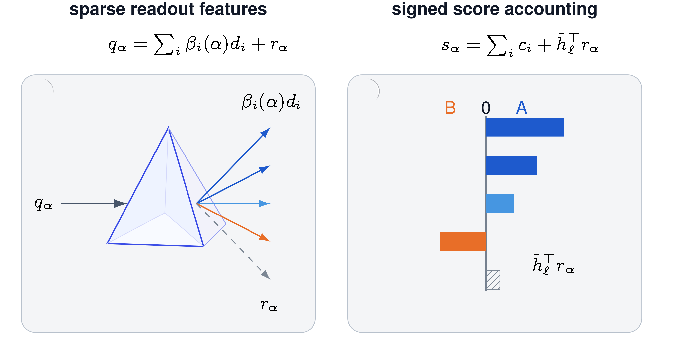
\includegraphics[width=\columnwidth]{figures/schematic_tikz/readout_query_one_column.pdf}
    \vspace{-0.8\baselineskip}
    \caption{\textbf{Local score decomposition schematic.}
    A vocabulary-mean or other selected contrast is decomposed into readout features learned
    from unembedding rows. Positive/negative bars support the first/comparison
    side; each signed term multiplies a direction coefficient by \(h\)'s readout
    feature projection. Hatching marks reconstruction error; raw token logits
    also include a shared offset.}
    \label{fig:readout-query-schematic}
\end{figure}

Fix a hidden state \(h\) and any selected readout direction
\(q_\alpha=\sum_{t\in\mathcal{V}}\alpha_t w_t\). Substituting the SAE
reconstruction gives
\[
\begin{aligned}
    s_\alpha(h)
    &= h^\top q_\alpha \\
    &=
    \left(\sum_{t\in\mathcal{V}} \alpha_t\right) h^\top\mu \\
    &\quad + \sum_{i=1}^{D}
        \left(\sum_{t\in\mathcal{V}} \alpha_t z_{t,i}\right) h^\top d_i \\
    &\quad + h^\top \sum_{t\in\mathcal{V}} \alpha_t r_t .
\end{aligned}
\]
For readout feature \(i\), define its direction coefficient and signed feature
contribution:
\[
    \beta_i(\alpha)=\sum_{t\in\mathcal{V}} \alpha_t z_{t,i},
    \qquad
    c_i(h,\alpha)=\beta_i(\alpha)\,p_i(h).
\]
Here \(\beta_i(\alpha)\) is fixed by the selected direction and readout SAE,
while \(p_i(h)\) varies with context; when \(q=q_\alpha\) is clear, we write
\(\beta_i(q)\). A feature matters locally when both factors are large in
magnitude. The profile coordinate alone is not support or opposition until a
selected readout direction is fixed
(Appendix~\ref{app:global-readout-feature-profiles}).

For a selected score, let
\[
\begin{aligned}
    s_{\mu}&=\left(\sum_t\alpha_t\right)h^\top\mu,\\
    s_{\mathrm{feat}}&=\sum_i c_i(h,\alpha),\\
    s_{\mathrm{recon}}&=s_{\mu}+s_{\mathrm{feat}} .
\end{aligned}
\]
The sparse account leaves residual
\[
\begin{aligned}
    s_{\mathrm{exact}}&=s_\alpha(h),\\
    \epsilon
    &=
    s_{\mathrm{exact}}-s_{\mathrm{recon}}\\
    &=
    h^\top\sum_{t\in\mathcal{V}}\alpha_t r_t .
\end{aligned}
\]
Positive terms raise the chosen score and negative terms lower it. For signed
contrasts, positive values support the first side and negative values support
the comparison side.

\subsection{Common Target Coefficients}
\label{sec:method-target-coefficients}

\Cref{tab:method-special-cases} lists \(\beta_i(\alpha)\) for common score
families. Write
\(\bar{z}_{\mathcal{A},i}=|\mathcal{A}|^{-1}\sum_{a\in\mathcal{A}}z_{a,i}\)
for the uniform average of feature \(i\)'s sparse coefficient over token group
\(\mathcal{A}\). For top-competitor margins, write
\(\bar{w}_{\pi,\mathcal{R}}=\sum_{r\in\mathcal{R}}\pi_r w_r\) and
\(\bar{z}_{\pi,\mathcal{R},i}=\sum_{r\in\mathcal{R}}\pi_r z_{r,i}\).

\begin{table}[H]
\caption{\textbf{Target choices and their sparse-feature coefficients.}
Rows instantiate the selected readout direction \(q_\alpha\) and corresponding
direction coefficient \(\beta_i(\alpha)\). Barred quantities denote uniform
token-set averages or competitor-weighted averages.}
\label{tab:method-special-cases}
\centering
\footnotesize
\setlength{\tabcolsep}{3pt}
\renewcommand{\arraystretch}{1.14}
\begin{tabularx}{\linewidth}{@{}>{\RaggedRight\arraybackslash}p{0.34\linewidth}Z Z@{}}
\toprule
Score or contrast & \(q_\alpha\) & \(\beta_i(\alpha)\) \\
\midrule
\textbf{Token score} & \(w_A\) & \(z_{A,i}\) \\
\addlinespace[1pt]
\textbf{Vocabulary-mean contrast} & \(w_A-\bar{w}_{\mathcal{V}}\) &
\(z_{A,i}-\bar{z}_{\mathcal{V},i}\) \\
\addlinespace[1pt]
\textbf{Logit difference} & \(w_A-w_B\) & \(z_{A,i}-z_{B,i}\) \\
\addlinespace[1pt]
\textbf{Group contrast} &
\(\bar{w}_{\mathcal{A}}-\bar{w}_{\mathcal{B}}\) &
\(\bar{z}_{\mathcal{A},i}-\bar{z}_{\mathcal{B},i}\) \\
\addlinespace[1pt]
\textbf{Top-competitor margin} &
\(w_u-\bar{w}_{\pi,\mathcal{R}}\) &
\(z_{u,i}-\bar{z}_{\pi,\mathcal{R},i}\) \\
\bottomrule
\end{tabularx}
\end{table}

For zero-sum contrasts and margins, the shared offset cancels. This includes
competitor margins because their weights satisfy
\(\sum_{r\in\mathcal{R}}\pi_r=1\).

\subsection{Reading and Gating Local Score Accounts}
\label{sec:method-reading-local-accounts}

A displayed local score account reports the selected readout score, exact score
\(s_{\mathrm{exact}}\), reconstructed score \(s_{\mathrm{recon}}\), feature sum
\(s_{\mathrm{feat}}\), offset term \(s_\mu\) when present, residual
\(\epsilon\), relative reconstruction error, and sign status for signed
contrasts. We compute relative reconstruction error as
\[
    \rho(h,\alpha)=
    \frac{|\epsilon|}{|s_{\mathrm{exact}}|+\delta},
    \qquad
    \delta=0.5\ \text{logit}.
\]
Small \(|\epsilon|\) or \(\rho\) indicates that the feature sum, plus offset
when present, reconstructs the chosen score. For signed contrasts, side-specific
interpretation is evidence-bearing only when \(s_{\mathrm{recon}}\) and
\(s_{\mathrm{exact}}\) agree in sign.

Figures may truncate small bars, but quantitative reconstructions use the full
feature sum. Claims remain tied to feature ids, signed contributions, and
residuals; labels are descriptive summaries of high-coefficient vocabulary rows,
following sparse-feature evaluation practice
\citep{karvonen2025saebench,makelov2024principled}.
